%-------------------------------------------------------------------------
% c-questionnements-info-S1.tex
%-------------------------------------------------------------------------

%-------------------------------------------------------------------------
\documentclass[11pt,a4paper,colorlinks,breaklinks]{article}
%-------------------------------------------------------------------------

%-------------------------------------------------------------------------
\usepackage{calc}
\usepackage[text={16cm,23cm},centering=true,showframe=false]{geometry}
\usepackage{fancybox,fancyvrb,fancyhdr,lastpage,lineno,import}
\usepackage{longtable,multirow}
\usepackage{xcolor,graphics,xmpmulti,pgf,pgfpages,tikz,wrapfig}
\usepackage{colortbl,color}
\usepackage{amsmath,amssymb,amsfonts}
\usepackage{hyperref,multimedia,rotating,framed,pstricks}
\usepackage{listings,index}
%
%---- pdflatex
%\usepackage[T1]{fontenc}
%\usepackage[utf8]{inputenc}
%---- xelatex
\usepackage{fontspec}
%
\usepackage[french]{minitoc}
\usepackage[french]{babel}
\usepackage[french]{nomencl}
\usepackage[framed,hyperref,standard]{ntheorem}
\usepackage{eurosym,pifont}
%-------------------------------------------------------------------------

%-------------------------------------------------------------------------
\definecolor{blanc}{RGB}{255,255,255}
\definecolor{orange}{RGB}{234,138,0}
\definecolor{bleu}{RGB}{144,209,223}
\definecolor{rose}{RGB}{233,96,124}
\definecolor{beige}{RGB}{247,244,241}
\definecolor{violet}{RGB}{159,159,202}
\definecolor{vert}{RGB}{162,169,63}
\definecolor{marron}{RGB}{193,181,162}
\definecolor{noir}{RGB}{62,61,64}
%-------------------------------------------------------------------------

%-------------------------------------------------------------------------
\usetikzlibrary{mindmap,backgrounds,shapes,decorations.text}
%-------------------------------------------------------------------------

%-------------------------------------------------------------------------
\input{sigle}
%-------------------------------------------------------------------------

%-------------------------------------------------------------------------
\lstset
{
language=Python,
basicstyle=\ttfamily,
identifierstyle=\ttfamily,
keywordstyle=\color{blue}\ttfamily,
commentstyle=\color{gray}\ttfamily,
stringstyle=\color{green}\ttfamily,
showstringspaces=false,
extendedchars=true,
numbers=left, 
numberstyle=\color{blue}\tiny,
frame=lines,
linewidth=0.95\textwidth,
xleftmargin=5mm
} 
%-------------------------------------------------------------------------

%-------------------------------------------------------------------------
\pgfdeclareimage[width=3cm,interpolate=true]{logo-enib}{logo-enib}
%-------------------------------------------------------------------------

%-------------------------------------------------------------------------
\pagestyle{fancy}
\fancyhead{}
\fancyhead[L]{\pgfuseimage{logo-enib}}
\fancyhead[C]{Informatique S1}
\fancyhead[R]{\thepage/\pageref{LastPage}}
\fancyfoot{}
\fancyfoot[L]{}
\fancyfoot[C]{}
\fancyfoot[R]{}
\setlength{\headheight}{40pt}
\setlength{\footskip}{38pt}
\renewcommand{\headrulewidth}{0pt}
\renewcommand{\footrulewidth}{0pt}
%-------------------------------------------------------------------------

%-------------------------------------------------------------------------
\newtheorem{question}{\color{blue}Q}[section]
%-------------------------------------------------------------------------

%-------------------------------------------------------------------------
\def\ga{\textsc{ga}}   
\def\bu{\textsc{bu}} 
\def\zo{\textsc{zo}} 
\def\meu{\textsc{meu}} 
\def\coeur{{\color{red}\heartsuit}}
%-------------------------------------------------------------------------

%-------------------------------------------------------------------------
\newcommand{\hexagone}[2]
{\draw[color=blue,fill=lightgray] (#1,#2) -- ({#1+1},#2) -- ({#1+3/2},{#2+sqrt(3)/2}) -- 
({#1+1},{#2+sqrt(3)}) -- (#1,{#2+sqrt(3)}) -- ({#1-1/2},{#2+sqrt(3)/2}) -- cycle;}
%-------------------------------------------------------------------------

%-------------------------------------------------------------------------
\graphicspath{{../fig/}}
%-------------------------------------------------------------------------

%-------------------------------------------------------------------------
\fvset
{
fontsize=\footnotesize,
numbers=left,
numbersep=5pt,
frame=lines
}  
%-------------------------------------------------------------------------

%-------------------------------------------------------------------------
\begin{document}
%-------------------------------------------------------------------------

%-------------------------------------------------------------------------
\begin{titlepage}
%-------------------------------------------------------------------------

%-------------------------------------------------------------------------
\thispagestyle{fancy}
\lhead{\hspace*{-2em}\begin{minipage}{5cm}
\includegraphics[width=5cm]{logo-enib}\end{minipage}}
\rhead{Cours d'Informatique S1}
\setlength{\headheight}{79pt}
\setlength{\footskip}{20pt}
\renewcommand{\headrulewidth}{0pt}
\renewcommand{\footrulewidth}{0pt}
%-------------------------------------------------------------------------

\begin{center}
{\huge\bf Initiation à l'algorithmique}\\[5mm]
{\huge\sc Solutions des questionnements de cours}\\[1cm]
\href{http://www.enib.fr/~tisseau}{\Large\sc Jacques TISSEAU}\\[3mm]
\href{http://www.enib.fr}{Ecole nationale d'ingénieurs de Brest}\\
\href{http://www.cerv.fr}{Centre européen de réalité virtuelle}\\
\href{mailto:tisseau@enib.fr}{\tt tisseau@enib.fr}
\end{center}
\vspace*{1cm}

{\footnotesize\vspace*{1.5mm}
\noindent Avec la participation de 
{\sc Romain Bénard}, 
{\sc Stéphane Bonneaud}, {\sc Cédric Buche},
{\sc Gireg Desmeulles}, {\sc Céline Jost}, 
{\sc Sébastien Kubicki}, {\sc Eric Maisel}, 
{\sc Aléxis Nédélec}, {\sc Marc Parenthoën} et 
{\sc Cyril Septseault}.
}
\null\vfill

\noindent \noindent Ce document regroupe les solutions, testées avec \python\ 3.2.2,
des questionnements du cours d'Infor\-ma\-tique 
d'informatique 
du $1^{er}$ semestre (S1) de l'Ecole Nationale d'Ingénieurs 
de Brest (ENIB : \href{http://www.enib.fr}{\tt www.enib.fr}).
Ils complètent les notes de cours « Initiation à l'algorithmique ».
$$\fbox{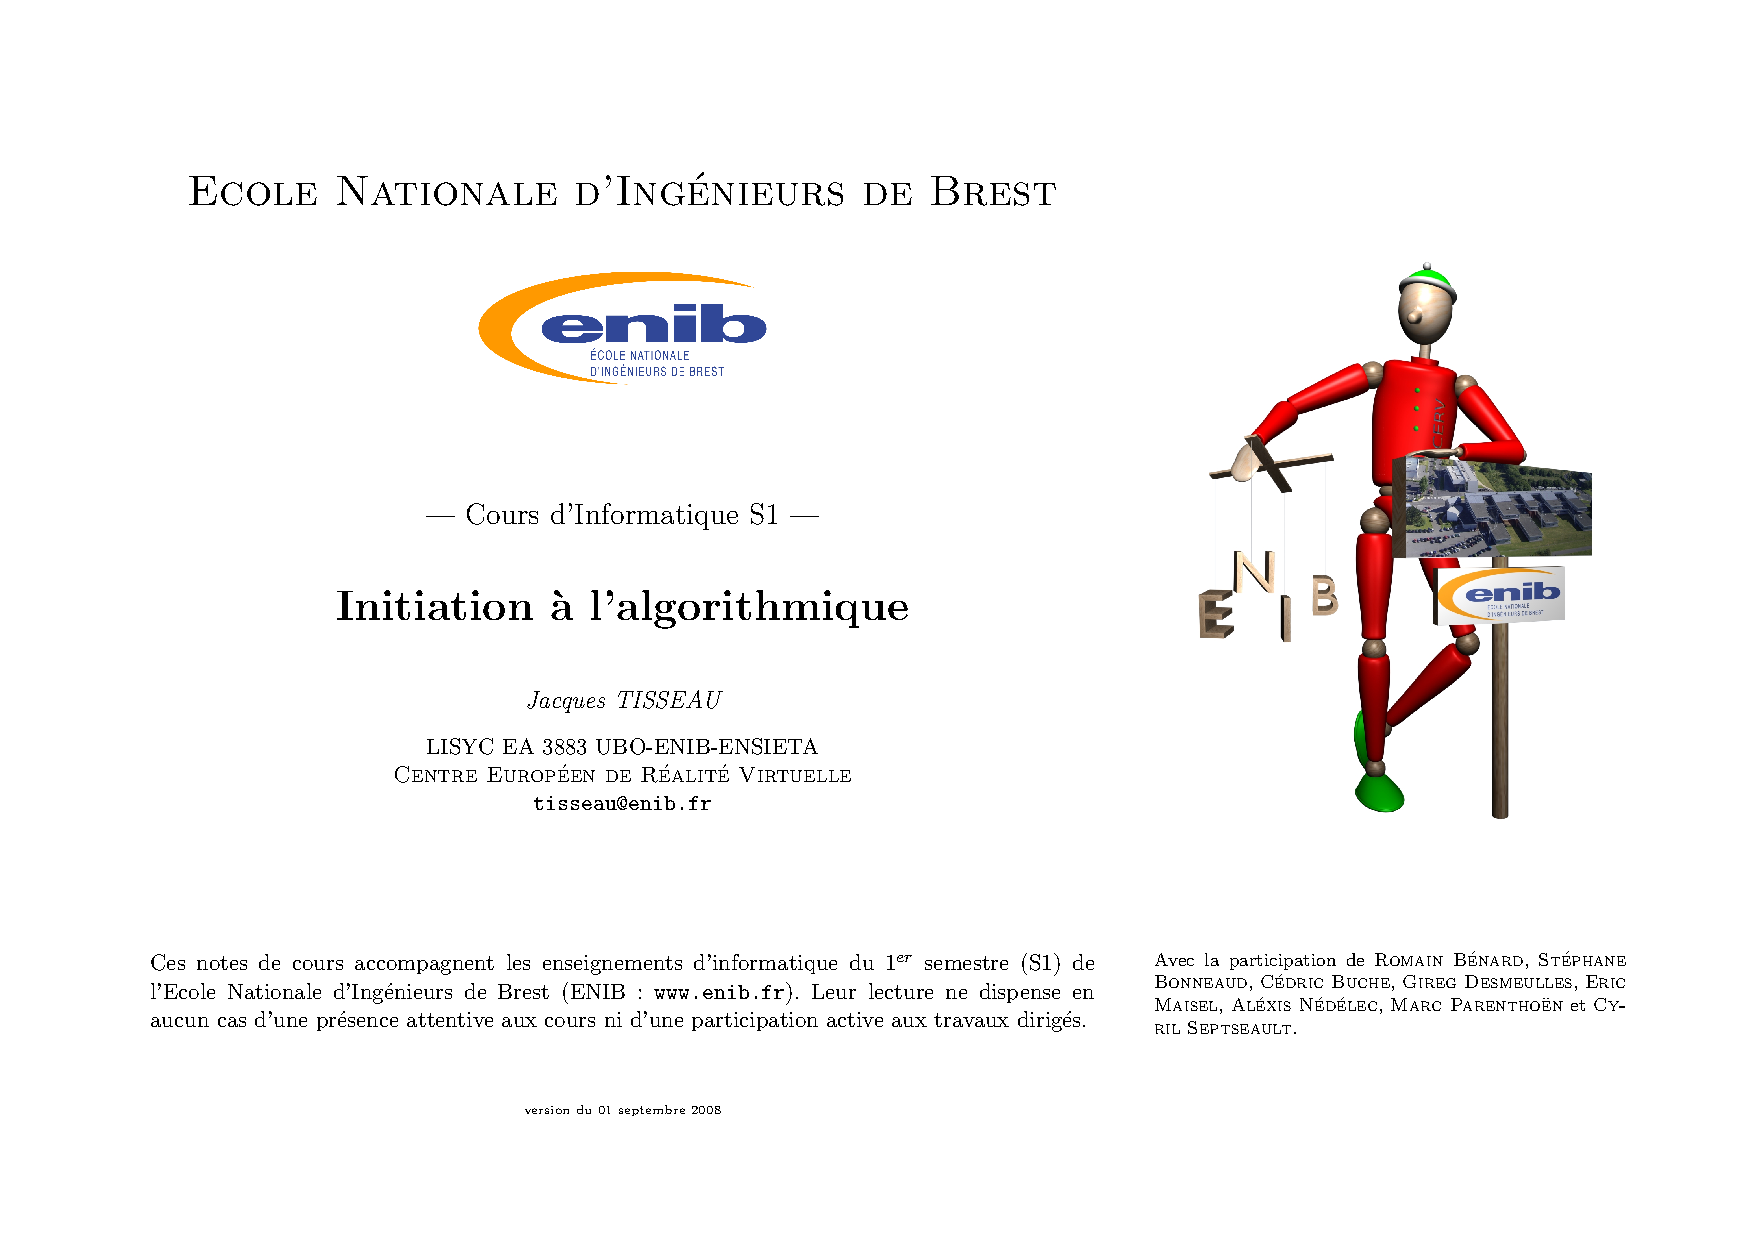
\includegraphics[width=14cm,page=1]{../../../../pdf/cours/info-S1.pdf}}$$
\centerline{\footnotesize
{\bf Tisseau J.},{\em Initiation à l'algorithmique}, ENIB, cours d'Informatique S1, Brest, 2009-2014.
}
\null\vfill

\centerline{\tiny version du \today}

\end{titlepage}
%-------------------------------------------------------------------------


%-------------------------------------------------------------------------
\pagestyle{fancy}
\fancyhead{}
\fancyhead[L]{\begin{minipage}{3cm}
\includegraphics[width=3cm]{logo-enib}\end{minipage}}
\fancyhead[C]{Informatique S1}
\fancyhead[R]{\thepage/\pageref{LastPage}}
\fancyfoot{}
\fancyfoot[L]{}
\fancyfoot[C]{}
\fancyfoot[R]{}
\setlength{\headheight}{47pt}
\setlength{\footskip}{38pt}
\renewcommand{\headrulewidth}{0pt}
\renewcommand{\footrulewidth}{0pt}
%-------------------------------------------------------------------------

%-------------------------------------------------------------------------
\setcounter{tocdepth}{2}
\tableofcontents
%-------------------------------------------------------------------------

%-------------------------------------------------------------------------
\newpage
%\setcounter{section}{0}
\section{Introduction}\label{sec:introduction}
%-------------------------------------------------------------------------
Ce document regroupe uniquement les codes sources \python\ correspondant 
aux questionnements \cite{questionnements} du cours d'initiation à
l'algorithmique \cite{cours} de l'\enib\ et non les méthodes 
et vérifications associées telles que le préconise la démarche \mvr\ \cite{mvr}.

Cette démarche, dite \mvr{} pour Méthode-Vérification-Résultat, est structurée en 3 étapes : 
\begin{enumerate}
\item on commence par expliciter la méthode générique qui permet de résoudre 
	des problèmes équivalents à celui qui est posé 
	(étape M comme Méthode);

\item on explicite ensuite une technique alternative ou complémentaire connue
	qui permettra de vérifier le résultat obtenu en appliquant la méthode générique 
	précédente
	(étape V comme Vérification).

\item enfin, on applique la méthode générique (M) et la technique de vérification (V)
	au cas particulier de l'énoncé pour obtenir le résultat attendu par l'exercice
	(étape R comme Résultat);
\end{enumerate}

La démarche complète est détaillée en cours, au cas par cas, lors de la correction
de ces questionnements.

%-------------------------------------------------------------------------
\newpage
%\setcounter{section}{1}
\section{Qu'est-ce que l'algorithmique ?}\label{sec:algo}
%-------------------------------------------------------------------------
	\VerbatimInput{q-introduction.py}
	
%-------------------------------------------------------------------------
\newpage
%\setcounter{section}{2}
\section{Qu'est-ce que l'affectation ?}\label{sec:affectation}
%-------------------------------------------------------------------------
	\VerbatimInput{q-affectation.py}
	
%-------------------------------------------------------------------------
\newpage
%\setcounter{section}{3}
\section{Comment calcule-t-on avec des opérateurs booléens ?}\label{sec:booleens}
%-------------------------------------------------------------------------
	\VerbatimInput{q-booleens.py}

%-------------------------------------------------------------------------
\newpage
%\setcounter{section}{4}
\section{Comment coder un nombre ?}\label{sec:codage}
%-------------------------------------------------------------------------
	\VerbatimInput{q-codage.py}

%-------------------------------------------------------------------------
\newpage
%\setcounter{section}{5}
\section{Qu'est-ce qu'un test ?}\label{sec:tests}
%-------------------------------------------------------------------------
	\VerbatimInput{q-tests.py}

%-------------------------------------------------------------------------
\newpage
%\setcounter{section}{6}
\section{Comment construit-on une boucle ?}\label{sec:boucles}
%-------------------------------------------------------------------------
	\VerbatimInput{q-boucles.py}

%-------------------------------------------------------------------------
\newpage
%\setcounter{section}{7}
\section{Comment imbriquer des boucles ?}\label{sec:boucles-imbriquees}
%-------------------------------------------------------------------------
	\VerbatimInput{q-boucles-imbriquees.py}

%-------------------------------------------------------------------------
\newpage
%\setcounter{section}{8}
\section{Comment spécifier une fonction ?}\label{sec:specification}
%-------------------------------------------------------------------------
	\VerbatimInput{q-introduction.py}

%-------------------------------------------------------------------------
\newpage
%\setcounter{section}{9}
\section{Qu'est-ce que la récursivité ?}\label{sec:recursivite}
%-------------------------------------------------------------------------
	\VerbatimInput{q-recursivite.py}

%-------------------------------------------------------------------------
\newpage
%\setcounter{section}{10}
\section{Comment trier une séquence ?}\label{sec:sequences}
%-------------------------------------------------------------------------
	\VerbatimInput{q-sequences.py}

%-------------------------------------------------------------------------
\newpage
%\setcounter{section}{11}
\section{Tout en un ?}\label{sec:conclusion}
%-------------------------------------------------------------------------
	\VerbatimInput{q-conclusion.py}

%-------------------------------------------------------------------------
\newpage
\begin{thebibliography}{99}\label{annexe:biblio}
\addcontentsline{toc}{section}{Références}
\bibitem{cours} Tisseau J., \emph{Initiation à l'algorithmique. \href{http://www.enib.fr/~tisseau/pdf/course/info-S1.pdf}{Cours}}, \enib, 2009-2014
\bibitem{td} Tisseau J., \emph{Initiation à l'algorithmique. \href{http://www.enib.fr/~tisseau/pdf/course/td-info-S1.pdf}{Travaux dirigés}}, \enib, 2009-2014
\bibitem{questionnements} Tisseau J., \emph{Initiation à l'algorithmique. \href{http://www.enib.fr/~tisseau/pdf/course/q-info-S1.pdf}{Questionnments de cours}}, \enib, 2011-2014
\bibitem{mvr} Tisseau J., Nédélec A., Parenthoën M., \emph{Initiation à l'algorithmique. \href{http://www.enib.fr/~tisseau/pdf/course/mvr-paper.pdf}{La démarche \mvr : méthode, vérification, résultat}}, \enib, 2011-2014
\end{thebibliography}
%-------------------------------------------------------------------------

\label{fin}
%-------------------------------------------------------------------------
\end{document}
%-------------------------------------------------------------------------
